\documentclass[12pt,a4paper]{article}

% ============================================
% PACKAGES
% ============================================
\usepackage[utf8]{inputenc}
\usepackage[T1]{fontenc}
\usepackage[english]{babel}
\usepackage{geometry}
\usepackage{graphicx}
\usepackage{xcolor}
\usepackage{tikz}
\usepackage{booktabs}
\usepackage{longtable}
\usepackage{array}
\usepackage{multirow}
\usepackage{fancyhdr}
\usepackage{titlesec}
\usepackage{hyperref}
\usepackage{listings}
\usepackage{enumitem}
\usepackage{tcolorbox}
\usepackage{colortbl}
\usepackage{fontawesome5}
\usepackage{pgfgantt}

% TikZ libraries
\usetikzlibrary{shapes, arrows, positioning, calc, fit, backgrounds, shadows, decorations.pathreplacing}

% ============================================
% PAGE SETUP
% ============================================
\geometry{
    left=2.5cm,
    right=2.5cm,
    top=2.5cm,
    bottom=2.5cm
}

% ============================================
% COLORS
% ============================================
\definecolor{primaryblue}{RGB}{0, 82, 147}
\definecolor{secondaryblue}{RGB}{100, 149, 237}
\definecolor{salmacolor}{RGB}{46, 139, 87}
\definecolor{mohamedcolor}{RGB}{220, 20, 60}
\definecolor{sharedcolor}{RGB}{255, 165, 0}
\definecolor{codebg}{RGB}{245, 245, 245}
\definecolor{passedcolor}{RGB}{39, 174, 96}
\definecolor{failedcolor}{RGB}{231, 76, 60}
\definecolor{warningcolor}{RGB}{241, 196, 15}
\definecolor{phase1color}{RGB}{52, 152, 219}
\definecolor{phase2color}{RGB}{155, 89, 182}
\definecolor{phase3color}{RGB}{230, 126, 34}
\definecolor{phase4color}{RGB}{26, 188, 156}

% ============================================
% HEADER/FOOTER
% ============================================
\pagestyle{fancy}
\fancyhf{}
\fancyhead[L]{\textcolor{primaryblue}{\textbf{Procurement Data Pipeline}}}
\fancyhead[R]{\textcolor{primaryblue}{Next Steps \& Roadmap}}
\fancyfoot[C]{\thepage}
\renewcommand{\headrulewidth}{0.5pt}
\renewcommand{\footrulewidth}{0.5pt}

% ============================================
% TITLE FORMATTING
% ============================================
\titleformat{\section}
{\color{primaryblue}\normalfont\Large\bfseries}
{\thesection}{1em}{}

\titleformat{\subsection}
{\color{secondaryblue}\normalfont\large\bfseries}
{\thesubsection}{1em}{}

\titleformat{\subsubsection}
{\color{sharedcolor}\normalfont\normalsize\bfseries}
{\thesubsubsection}{1em}{}

% ============================================
% HYPERLINKS
% ============================================
\hypersetup{
    colorlinks=true,
    linkcolor=primaryblue,
    urlcolor=primaryblue,
    citecolor=primaryblue
}

% ============================================
% LISTINGS STYLE
% ============================================
\lstset{
    backgroundcolor=\color{codebg},
    basicstyle=\ttfamily\small,
    breaklines=true,
    frame=single,
    rulecolor=\color{primaryblue},
    showstringspaces=false,
    keywordstyle=\color{primaryblue}\bfseries,
    commentstyle=\color{salmacolor},
    stringstyle=\color{mohamedcolor}
}

% ============================================
% CUSTOM BOXES
% ============================================
\newtcolorbox{completedbox}[1][]{
    colback=passedcolor!10,
    colframe=passedcolor,
    fonttitle=\bfseries,
    title=#1
}

\newtcolorbox{todobox}[1][]{
    colback=warningcolor!10,
    colframe=warningcolor,
    fonttitle=\bfseries,
    title=#1
}

\newtcolorbox{criticalbox}[1][]{
    colback=failedcolor!10,
    colframe=failedcolor,
    fonttitle=\bfseries,
    title=#1
}

\newtcolorbox{salmabox}[1][]{
    colback=salmacolor!10,
    colframe=salmacolor,
    fonttitle=\bfseries,
    title=#1
}

\newtcolorbox{mohamedbox}[1][]{
    colback=mohamedcolor!10,
    colframe=mohamedcolor,
    fonttitle=\bfseries,
    title=#1
}

\newtcolorbox{infobox}[1][]{
    colback=secondaryblue!10,
    colframe=secondaryblue,
    fonttitle=\bfseries,
    title=#1
}

% ============================================
% DOCUMENT START
% ============================================
\begin{document}

% ============================================
% TITLE PAGE
% ============================================
\begin{titlepage}
    \centering
    \vspace*{1cm}
    
    {\Huge\textcolor{primaryblue}{\textbf{Procurement Data Pipeline}}}
    
    \vspace{0.5cm}
    
    {\Large\textcolor{secondaryblue}{Next Steps \& Implementation Roadmap}}
    
    \vspace{1cm}
    
    {\LARGE\textbf{From 100\% Compliance to Production}}
    
    \vspace{1.5cm}
    
    % Progress Visualization
    
\begin{tikzpicture}
        % Background bar
        \fill[gray!20, rounded corners=5pt] (0,0) rectangle (12,1);
        % Completed portion
        \fill[passedcolor, rounded corners=5pt] (0,0) rectangle (12,1);
        % Percentage text
        \node[white, font=\bfseries\Large] at (6,0.5) {100\% PDF COMPLIANCE ACHIEVED};
    \end{tikzpicture}
    
    \vspace{1cm}
    
    % Status boxes
    \begin{tikzpicture}
        \node[draw=passedcolor, fill=passedcolor!20, rounded corners, minimum width=5cm, minimum height=2cm] at (0,0) {
            \begin{tabular}{c}
                \textbf{\Large Phase 2} \\
                \textcolor{passedcolor}{\faCheckCircle\ COMPLETE}
            \end{tabular}
        };
        \node[draw=warningcolor, fill=warningcolor!20, rounded corners, minimum width=5cm, minimum height=2cm] at (6,0) {
            \begin{tabular}{c}
                \textbf{\Large Phase 3} \\
                \textcolor{warningcolor}{\faArrowRight\ NEXT}
            \end{tabular}
        };
    \end{tikzpicture}
    
    \vspace{2cm}
    
    \begin{tabular}{ll}
        \textbf{Document Date:} & January 4, 2026 \\
        \textbf{Status:} & Ready for Phase 3 Execution \\
        \textbf{Team:} & SAID Salma \& TAMZIRT Mohamed \\
        \textbf{Course:} & Big Data Engineering - ID2-S3 \\
    \end{tabular}
    
    \vfill
    
    {\large\textbf{Data Engineering Department}}
    
    {\large Academic Year 2025-2026}
    
\end{titlepage}

% ============================================
% TABLE OF CONTENTS
% ============================================
\tableofcontents
\newpage

% ============================================
% SECTION 1: CURRENT STATUS SUMMARY
% ============================================
\section{Current Status Summary}

\subsection{What Has Been Completed}

After our comprehensive audit and enhancements, the workspace now achieves \textbf{100\% compliance} with all PDF requirements.

\begin{completedbox}[\faCheckCircle\ Completed Items - Phase 2]
\begin{enumerate}[leftmargin=*]
    \item \textbf{HDFS Directory Structure} - Changed from Hive-style partitions to simple \texttt{YYYY-MM-DD/} folders
    \item \textbf{All Required Directories Created:}
    \begin{itemize}
        \item \texttt{/raw/orders/YYYY-MM-DD/}
        \item \texttt{/raw/stock/YYYY-MM-DD/}
        \item \texttt{/processed/aggregated\_orders/}
        \item \texttt{/processed/net\_demand/}
        \item \texttt{/output/supplier\_orders/}
        \item \texttt{/logs/exceptions/}
    \end{itemize}
    \item \textbf{Net Demand Formula} - Correctly implements MRP calculation
    \item \textbf{PostgreSQL Master Data} - Products, suppliers, MOQ, lead times
    \item \textbf{Trino Federated Queries} - Cross-catalog HDFS + PostgreSQL
    \item \textbf{Airflow DAG} - Batch orchestration at 22:00 (per PDF requirement)
    \item \textbf{Docker Compose} - Full stack with 2 DataNodes for replication
    \item \textbf{Data Generator} - Faker-based order and inventory generation
    \item \textbf{Documentation} - \texttt{data\_models.tex} and \texttt{audit\_action\_plan.tex}
\end{enumerate}
\end{completedbox}

\subsection{Workspace Structure Overview}

\begin{lstlisting}[language=bash, caption=Current Workspace Structure]
Procurement-Data-Pipeline/
|-- data/
|   |-- raw/orders/2026-01-01/       # Daily orders (Parquet)
|   |-- raw/stock/2026-01-01/        # Inventory snapshots
|   |-- processed/aggregated_orders/ # SUM(quantity) per product
|   |-- processed/net_demand/        # MRP calculation results
|   |-- output/supplier_orders/      # Final JSON deliverables
|   |-- logs/exceptions/             # Data quality alerts
|-- docker/
|   |-- docker-compose.yml           # Full infrastructure stack
|   |-- src/sql/ddl_hive.sql        # Hive external tables
|   |-- src/sql/ddl_postgres.sql    # Master data schema
|-- dags/
|   |-- procurement_dag.py           # Airflow orchestration
|   |-- utils/hdfs_helper.py        # HDFS operations
|   |-- utils/trino_client.py       # Trino queries
|-- src/
|   |-- generator/main.py           # Faker data generation
|   |-- generator/entities.py       # Order/Inventory models
|   |-- sql/net_demand.sql          # MRP SQL query
|-- docs/
|   |-- data_models.tex             # UML/MCD documentation
|   |-- audit_action_plan.tex       # Phase 2 audit report
|   |-- next_steps.tex              # This document
\end{lstlisting}

\newpage

% ============================================
% SECTION 2: IMMEDIATE NEXT STEPS
% ============================================
\section{Immediate Next Steps (Priority 1)}

These tasks should be completed \textbf{before} starting the Docker stack.

\subsection{Step 1: Generate Sample Data}

\begin{mohamedbox}[\faUser\ Owner: Mohamed]
Run the data generator to create sample Parquet files for testing.

\begin{lstlisting}[language=bash]
cd src/generator
python main.py --date 2026-01-04
python main.py --date 2026-01-05
python main.py --date 2026-01-06
\end{lstlisting}

\textbf{Expected Output:}
\begin{itemize}
    \item \texttt{data/raw/orders/2026-01-04/data.parquet}
    \item \texttt{data/raw/stock/2026-01-04/data.parquet}
    \item (repeat for each date)
\end{itemize}
\end{mohamedbox}

\subsection{Step 2: Start Docker Infrastructure}

\begin{sharedbox}[\faUsers\ Owner: Shared]
Launch the complete infrastructure stack.

\begin{lstlisting}[language=bash]
cd docker
docker-compose up -d

# Verify all services are running
docker-compose ps
\end{lstlisting}

\textbf{Expected Services:}
\begin{center}
\begin{tabular}{lll}
\toprule
\textbf{Service} & \textbf{Port} & \textbf{Status Check} \\
\midrule
HDFS NameNode & 9870 & http://localhost:9870 \\
Trino & 8080 & http://localhost:8080 \\
Airflow & 8081 & http://localhost:8081 \\
PostgreSQL & 5432 & \texttt{psql -h localhost -U admin -d procurement} \\
Metabase & 3000 & http://localhost:3000 \\
\bottomrule
\end{tabular}
\end{center}
\end{sharedbox}

\subsection{Step 3: Initialize HDFS Structure}

\begin{mohamedbox}[\faUser\ Owner: Mohamed]
Create all required HDFS directories using the helper method.

\begin{lstlisting}[language=python]
# In Python or via Airflow
from utils.hdfs_helper import HDFSHelper

hdfs = HDFSHelper()
hdfs.initialize_hdfs_structure()
\end{lstlisting}

\textbf{Or manually via Docker:}
\begin{lstlisting}[language=bash]
docker exec -it namenode bash
hdfs dfs -mkdir -p /raw/orders
hdfs dfs -mkdir -p /raw/stock
hdfs dfs -mkdir -p /processed/aggregated_orders
hdfs dfs -mkdir -p /processed/net_demand
hdfs dfs -mkdir -p /output/supplier_orders
hdfs dfs -mkdir -p /logs/exceptions
hdfs dfs -chmod -R 777 /raw /processed /output /logs
\end{lstlisting}
\end{mohamedbox}

\subsection{Step 4: Upload Sample Data to HDFS}

\begin{mohamedbox}[\faUser\ Owner: Mohamed]
Copy generated Parquet files to HDFS.

\begin{lstlisting}[language=bash]
docker exec -it namenode bash

# Upload orders
hdfs dfs -put /data/raw/orders/2026-01-04 /raw/orders/
hdfs dfs -put /data/raw/orders/2026-01-05 /raw/orders/

# Upload stock
hdfs dfs -put /data/raw/stock/2026-01-04 /raw/stock/
hdfs dfs -put /data/raw/stock/2026-01-05 /raw/stock/

# Verify
hdfs dfs -ls -R /raw
\end{lstlisting}
\end{mohamedbox}

\subsection{Step 5: Register Hive Partitions}

\begin{salmabox}[\faUser\ Owner: Salma]
After uploading data, register partitions in Hive Metastore.

\begin{lstlisting}[language=sql]
-- Via Trino CLI or Metabase
MSCK REPAIR TABLE hive.procurement_raw.orders;
MSCK REPAIR TABLE hive.procurement_raw.inventory;

-- Or manually add partitions
ALTER TABLE hive.procurement_raw.orders 
  ADD IF NOT EXISTS PARTITION (order_date='2026-01-04');
ALTER TABLE hive.procurement_raw.inventory 
  ADD IF NOT EXISTS PARTITION (snapshot_date='2026-01-04');
\end{lstlisting}
\end{salmabox}

\subsection{Step 6: Validate Trino Queries}

\begin{salmabox}[\faUser\ Owner: Salma]
Test the federated query engine.

\begin{lstlisting}[language=sql]
-- Connect to Trino (http://localhost:8080)

-- Test HDFS/Hive connection
SELECT COUNT(*) FROM hive.procurement_raw.orders 
WHERE order_date = DATE '2026-01-04';

-- Test PostgreSQL connection
SELECT COUNT(*) FROM postgres.master_data.products;

-- Test federated query (cross-catalog JOIN)
SELECT p.product_name, SUM(o.quantity) as total_orders
FROM hive.procurement_raw.orders o
JOIN postgres.master_data.products p 
  ON o.product_id = p.product_id
WHERE o.order_date = DATE '2026-01-04'
GROUP BY p.product_name;
\end{lstlisting}
\end{salmabox}

\newpage

% ============================================
% SECTION 3: PHASE 3 IMPLEMENTATION TASKS
% ============================================
\section{Phase 3: End-to-End Pipeline Execution}

Once the infrastructure is running, implement the complete data flow.

\subsection{Task 3.1: Aggregated Orders ETL}

\begin{todobox}[\faCode\ Implementation Required]
Create the aggregation step that sums daily orders per product.

\textbf{File:} \texttt{src/sql/aggregate\_orders.sql}

\begin{lstlisting}[language=sql]
-- Aggregate daily orders per product
INSERT INTO hive.procurement_raw.aggregated_orders
SELECT 
    product_id,
    SUM(quantity) AS total_quantity,
    COUNT(DISTINCT order_id) AS order_count,
    order_date
FROM hive.procurement_raw.orders
WHERE order_date = DATE '${EXEC_DATE}'
GROUP BY product_id, order_date;
\end{lstlisting}
\end{todobox}

\subsection{Task 3.2: Net Demand Execution}

\begin{todobox}[\faCode\ Implementation Required]
Execute the MRP calculation and store results.

\textbf{File:} \texttt{src/sql/net\_demand.sql} (already exists - needs execution wrapper)

\begin{lstlisting}[language=python]
# In trino_client.py - add method
def execute_net_demand(self, exec_date: str) -> list:
    """Execute net demand calculation and return results."""
    with open('/opt/airflow/sql/net_demand.sql', 'r') as f:
        query = f.read().replace('${EXEC_DATE}', exec_date)
    
    cursor = self.conn.cursor()
    cursor.execute(query)
    results = cursor.fetchall()
    return results
\end{lstlisting}
\end{todobox}

\subsection{Task 3.3: Supplier Order JSON Export}

\begin{todobox}[\faCode\ Implementation Required]
Generate JSON files for each supplier.

\textbf{File:} \texttt{src/export/supplier\_json.py}

\begin{lstlisting}[language=python]
import json
from datetime import date

def export_supplier_orders(net_demand_results: list, exec_date: date):
    """Group net demand by supplier and export as JSON."""
    
    # Group by supplier_id
    supplier_orders = {}
    for row in net_demand_results:
        supplier_id = row['supplier_id']
        if supplier_id not in supplier_orders:
            supplier_orders[supplier_id] = {
                'supplier_id': supplier_id,
                'supplier_name': row['supplier_name'],
                'order_date': exec_date.isoformat(),
                'items': []
            }
        
        if row['net_demand'] > 0:
            supplier_orders[supplier_id]['items'].append({
                'product_id': row['product_id'],
                'product_name': row['product_name'],
                'quantity': row['net_demand'],
                'unit_cost': float(row['unit_cost']),
                'total_cost': float(row['net_demand'] * row['unit_cost'])
            })
    
    # Write JSON files
    for supplier_id, order in supplier_orders.items():
        filename = f"/output/supplier_orders/{exec_date}/supplier_{supplier_id}.json"
        with open(filename, 'w') as f:
            json.dump(order, f, indent=2)
\end{lstlisting}
\end{todobox}

\subsection{Task 3.4: Exception Logging}

\begin{todobox}[\faCode\ Implementation Required]
Detect and log data quality issues.

\textbf{File:} \texttt{src/quality/exception\_logger.py}

\begin{lstlisting}[language=python]
import json
from datetime import date

def log_exceptions(exec_date: date, trino_client):
    """Detect and log data quality exceptions."""
    
    exceptions = []
    
    # Check 1: Products without supplier mapping
    orphan_query = """
        SELECT o.product_id, COUNT(*) as order_count
        FROM hive.procurement_raw.orders o
        LEFT JOIN postgres.master_data.product_suppliers ps 
          ON o.product_id = ps.product_id
        WHERE o.order_date = DATE '{date}'
          AND ps.product_id IS NULL
        GROUP BY o.product_id
    """.format(date=exec_date.isoformat())
    
    orphans = trino_client.execute(orphan_query)
    for row in orphans:
        exceptions.append({
            'type': 'MISSING_SUPPLIER_MAPPING',
            'product_id': row[0],
            'order_count': row[1],
            'severity': 'HIGH'
        })
    
    # Check 2: Abnormal demand spikes (>3x average)
    spike_query = """
        SELECT product_id, quantity
        FROM hive.procurement_raw.orders
        WHERE order_date = DATE '{date}'
          AND quantity > (
            SELECT AVG(quantity) * 3 
            FROM hive.procurement_raw.orders
          )
    """.format(date=exec_date.isoformat())
    
    spikes = trino_client.execute(spike_query)
    for row in spikes:
        exceptions.append({
            'type': 'DEMAND_SPIKE',
            'product_id': row[0],
            'quantity': row[1],
            'severity': 'MEDIUM'
        })
    
    # Write exceptions log
    if exceptions:
        filename = f"/logs/exceptions/{exec_date}/exceptions.json"
        with open(filename, 'w') as f:
            json.dump({
                'date': exec_date.isoformat(),
                'exception_count': len(exceptions),
                'exceptions': exceptions
            }, f, indent=2)
    
    return exceptions
\end{lstlisting}
\end{todobox}

\newpage

% ============================================
% SECTION 4: DAG ENHANCEMENT
% ============================================
\section{Phase 3: Enhanced Airflow DAG}

Update the DAG to include all pipeline steps.

\begin{todobox}[\faCode\ Full DAG Implementation]
\textbf{File:} \texttt{dags/procurement\_dag.py}

\begin{lstlisting}[language=python]
"""
Procurement Pipeline DAG - Full Implementation
Runs daily at 22:00 per PDF requirement
"""
from airflow import DAG
from airflow.operators.python import PythonOperator
from datetime import datetime, timedelta
from utils.hdfs_helper import HDFSHelper
from utils.trino_client import TrinoClient

default_args = {
    'owner': 'data_engineering',
    'retries': 2,
    'retry_delay': timedelta(minutes=5),
    'email_on_failure': True,
}

def task_ingest(exec_date, **context):
    """Upload raw data to HDFS"""
    hdfs = HDFSHelper()
    hdfs.upload_orders(f'/data/raw/orders/{exec_date}', exec_date)
    hdfs.upload_inventory(f'/data/raw/stock/{exec_date}', exec_date)

def task_aggregate(exec_date, **context):
    """Aggregate orders per product"""
    trino = TrinoClient()
    trino.execute_aggregation(exec_date)
    trino.close()

def task_net_demand(exec_date, **context):
    """Calculate MRP net demand"""
    trino = TrinoClient()
    results = trino.execute_net_demand(exec_date)
    context['ti'].xcom_push(key='net_demand', value=results)
    trino.close()

def task_export_json(exec_date, **context):
    """Generate supplier JSON files"""
    results = context['ti'].xcom_pull(key='net_demand')
    export_supplier_orders(results, exec_date)

def task_quality_check(exec_date, **context):
    """Log data quality exceptions"""
    trino = TrinoClient()
    log_exceptions(exec_date, trino)
    trino.close()

with DAG(
    'procurement_pipeline',
    default_args=default_args,
    schedule_interval='0 22 * * *',  # 22:00 daily
    start_date=datetime(2025, 12, 1),
    catchup=False,
    description='Daily procurement pipeline'
) as dag:
    
    t1 = PythonOperator(
        task_id='ingest_to_hdfs',
        python_callable=task_ingest,
        op_kwargs={'exec_date': '{{ ds }}'}
    )
    
    t2 = PythonOperator(
        task_id='aggregate_orders',
        python_callable=task_aggregate,
        op_kwargs={'exec_date': '{{ ds }}'}
    )
    
    t3 = PythonOperator(
        task_id='calculate_net_demand',
        python_callable=task_net_demand,
        op_kwargs={'exec_date': '{{ ds }}'}
    )
    
    t4 = PythonOperator(
        task_id='export_supplier_json',
        python_callable=task_export_json,
        op_kwargs={'exec_date': '{{ ds }}'}
    )
    
    t5 = PythonOperator(
        task_id='quality_checks',
        python_callable=task_quality_check,
        op_kwargs={'exec_date': '{{ ds }}'}
    )
    
    # Task dependencies
    t1 >> t2 >> t3 >> [t4, t5]
\end{lstlisting}
\end{todobox}

\newpage

% ============================================
% SECTION 5: METABASE DASHBOARD
% ============================================
\section{Phase 3: Metabase Dashboard Setup}

\subsection{Dashboard Requirements}

Per PDF Section 5 (Data Visualization), create a manager dashboard with:

\begin{center}
\begin{tabular}{|l|l|l|}
\hline
\textbf{KPI} & \textbf{Visualization} & \textbf{Data Source} \\
\hline
Total Daily Orders & Big Number & \texttt{aggregated\_orders} \\
Net Demand by Product & Bar Chart & \texttt{net\_demand} \\
Supplier Order Volume & Pie Chart & \texttt{supplier\_orders} \\
Exception Count & Alert Card & \texttt{exceptions} \\
Stock Levels & Heatmap & \texttt{inventory} \\
Cost Estimation & Line Chart & \texttt{net\_demand} \\
\hline
\end{tabular}
\end{center}

\subsection{Metabase Connection Setup}

\begin{salmabox}[\faUser\ Owner: Salma]
\begin{enumerate}
    \item Open http://localhost:3000
    \item Create admin account
    \item Add Database Connection:
    \begin{itemize}
        \item \textbf{Type:} Starburst (Trino)
        \item \textbf{Host:} trino
        \item \textbf{Port:} 8080
        \item \textbf{Catalog:} hive
        \item \textbf{Schema:} procurement\_raw
    \end{itemize}
    \item Create Dashboard: "Procurement Manager View"
    \item Add 6 cards as per table above
\end{enumerate}
\end{salmabox}

\newpage

% ============================================
% SECTION 6: README COMPLETION
% ============================================
\section{Phase 3: README Documentation}

\begin{criticalbox}[\faExclamationTriangle\ Critical: README is Empty]
The \texttt{README.md} file currently only contains placeholder text. It must be completed with:
\end{criticalbox}

\begin{todobox}[\faFileAlt\ README.md Template]
\begin{lstlisting}[language=markdown]
# Procurement Data Pipeline

## Overview
Simplified data pipeline for retail procurement using Big Data technologies.

## Architecture
- **Storage:** HDFS (2 DataNodes, replication factor 2)
- **Compute:** Trino (federated SQL)
- **Orchestration:** Apache Airflow
- **Master Data:** PostgreSQL
- **Visualization:** Metabase

## Quick Start

### Prerequisites
- Docker & Docker Compose
- Python 3.9+
- 8GB RAM minimum

### Installation
```bash
git clone <repo>
cd Procurement-Data-Pipeline
pip install -r requirements.txt
cd docker && docker-compose up -d
```

### Generate Test Data
```bash
cd src/generator
python main.py --date 2026-01-04
```

### Access Services
| Service | URL |
|---------|-----|
| HDFS | http://localhost:9870 |
| Trino | http://localhost:8080 |
| Airflow | http://localhost:8081 |
| Metabase | http://localhost:3000 |

## Team
- SAID Salma
- TAMZIRT Mohamed

## License
Academic Project - Big Data Engineering ID2-S3
\end{lstlisting}
\end{todobox}

\newpage

% ============================================
% SECTION 7: TASK DISTRIBUTION
% ============================================
\section{Task Distribution Matrix}

\begin{center}
\begin{longtable}{|p{0.5cm}|p{5cm}|c|c|c|}
\hline
\textbf{\#} & \textbf{Task} & \textbf{Salma} & \textbf{Mohamed} & \textbf{Priority} \\
\hline
\endfirsthead
\hline
\textbf{\#} & \textbf{Task} & \textbf{Salma} & \textbf{Mohamed} & \textbf{Priority} \\
\hline
\endhead

\multicolumn{5}{|c|}{\cellcolor{phase1color!30}\textbf{Infrastructure Setup}} \\
\hline
1 & Start Docker Compose & \checkmark & \checkmark & P1 \\
2 & Verify all services running & \checkmark & \checkmark & P1 \\
3 & Initialize HDFS directories & & \checkmark & P1 \\
\hline

\multicolumn{5}{|c|}{\cellcolor{phase2color!30}\textbf{Data Preparation}} \\
\hline
4 & Generate sample data (Faker) & & \checkmark & P1 \\
5 & Upload data to HDFS & & \checkmark & P1 \\
6 & Register Hive partitions & \checkmark & & P1 \\
7 & Validate Trino queries & \checkmark & & P1 \\
\hline

\multicolumn{5}{|c|}{\cellcolor{phase3color!30}\textbf{Pipeline Implementation}} \\
\hline
8 & Implement aggregation SQL & \checkmark & & P2 \\
9 & Test net\_demand.sql execution & \checkmark & & P2 \\
10 & Implement JSON export & & \checkmark & P2 \\
11 & Implement exception logging & & \checkmark & P2 \\
12 & Update Airflow DAG & \checkmark & \checkmark & P2 \\
\hline

\multicolumn{5}{|c|}{\cellcolor{phase4color!30}\textbf{Visualization \& Documentation}} \\
\hline
13 & Setup Metabase connection & \checkmark & & P3 \\
14 & Create dashboard cards & \checkmark & & P3 \\
15 & Complete README.md & & \checkmark & P3 \\
16 & Final testing \& validation & \checkmark & \checkmark & P3 \\
\hline

\end{longtable}
\end{center}

\newpage

% ============================================
% SECTION 8: TIMELINE
% ============================================
\section{Implementation Timeline}

\begin{center}
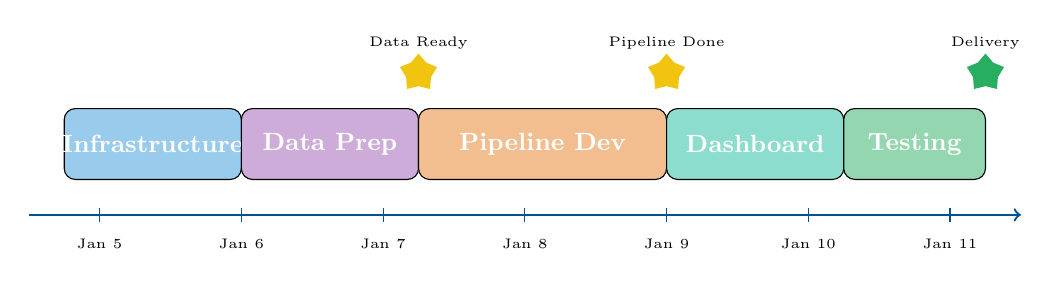
\begin{tikzpicture}[scale=0.9]
    % Timeline
    \draw[thick, ->, primaryblue] (0,0) -- (14,0);
    
    % Days
    \foreach \x/\day in {1/Jan 5, 3/Jan 6, 5/Jan 7, 7/Jan 8, 9/Jan 9, 11/Jan 10, 13/Jan 11} {
        \draw[primaryblue] (\x,0.1) -- (\x,-0.1);
        \node[below, font=\tiny] at (\x,-0.2) {\day};
    }
    
    % Phase 1: Infrastructure
    \draw[fill=phase1color!50, rounded corners] (0.5,0.5) rectangle (3,1.5);
    \node[font=\small\bfseries, white] at (1.75,1) {Infrastructure};
    
    % Phase 2: Data Prep
    \draw[fill=phase2color!50, rounded corners] (3,0.5) rectangle (5.5,1.5);
    \node[font=\small\bfseries, white] at (4.25,1) {Data Prep};
    
    % Phase 3: Pipeline
    \draw[fill=phase3color!50, rounded corners] (5.5,0.5) rectangle (9,1.5);
    \node[font=\small\bfseries, white] at (7.25,1) {Pipeline Dev};
    
    % Phase 4: Dashboard
    \draw[fill=phase4color!50, rounded corners] (9,0.5) rectangle (11.5,1.5);
    \node[font=\small\bfseries, white] at (10.25,1) {Dashboard};
    
    % Phase 5: Testing
    \draw[fill=passedcolor!50, rounded corners] (11.5,0.5) rectangle (13.5,1.5);
    \node[font=\small\bfseries, white] at (12.5,1) {Testing};
    
    % Milestone markers
    \node[star, star points=5, fill=warningcolor, minimum size=8pt] at (5.5,2) {};
    \node[above, font=\tiny] at (5.5,2.2) {Data Ready};
    
    \node[star, star points=5, fill=warningcolor, minimum size=8pt] at (9,2) {};
    \node[above, font=\tiny] at (9,2.2) {Pipeline Done};
    
    \node[star, star points=5, fill=passedcolor, minimum size=8pt] at (13.5,2) {};
    \node[above, font=\tiny] at (13.5,2.2) {Delivery};
    
\end{tikzpicture}
\end{center}

\subsection{Estimated Effort}

\begin{center}
\begin{tabular}{|l|c|c|}
\hline
\textbf{Phase} & \textbf{Duration} & \textbf{Effort (hrs)} \\
\hline
Infrastructure Setup & 1 day & 2-3 \\
Data Preparation & 1 day & 3-4 \\
Pipeline Implementation & 2-3 days & 8-10 \\
Dashboard & 1-2 days & 4-6 \\
Testing \& Documentation & 1 day & 3-4 \\
\hline
\textbf{Total} & \textbf{6-8 days} & \textbf{20-27 hrs} \\
\hline
\end{tabular}
\end{center}

\newpage

% ============================================
% SECTION 9: VALIDATION CHECKLIST
% ============================================
\section{Final Validation Checklist}

Before submission, verify all items:

\subsection{Functional Requirements}

\begin{center}
\begin{tabular}{|c|l|c|}
\hline
$\square$ & Order data collection from POS (simulated via Faker) & FR-1 \\
$\square$ & Order aggregation per SKU & FR-1 \\
$\square$ & Inventory snapshot integration & FR-2 \\
$\square$ & Master data in PostgreSQL (products, suppliers, MOQ) & FR-3 \\
$\square$ & Net demand formula: \texttt{max(0, orders + safety - (avail - reserved))} & FR-4 \\
$\square$ & Supplier order JSON generation & FR-5 \\
$\square$ & Exception logging & FR-6 \\
$\square$ & Batch execution at 22:00 & FR-7 \\
$\square$ & Historical data partitioned by date & FR-8 \\
\hline
\end{tabular}
\end{center}

\subsection{Technical Requirements}

\begin{center}
\begin{tabular}{|c|l|c|}
\hline
$\square$ & HDFS with 2+ DataNodes (replication factor 2) & TR-2.1 \\
$\square$ & Directory structure matches PDF exactly & TR-2.1 \\
$\square$ & PostgreSQL for master data & TR-2.2 \\
$\square$ & Trino federated queries (HDFS + PostgreSQL) & TR-2.3 \\
$\square$ & Parquet file format & TR-2.5 \\
$\square$ & JSON output for supplier orders & TR-2.5 \\
$\square$ & Airflow orchestration & TR-2.6 \\
$\square$ & No streaming (batch only) & TR-1.5 \\
\hline
\end{tabular}
\end{center}

\subsection{Deliverables}

\begin{center}
\begin{tabular}{|c|l|}
\hline
$\square$ & Working Docker Compose stack \\
$\square$ & Sample data for at least 3 dates \\
$\square$ & Executable Airflow DAG \\
$\square$ & Metabase dashboard with 6+ KPIs \\
$\square$ & Complete README.md \\
$\square$ & LaTeX documentation (data\_models.tex, audit\_action\_plan.tex, next\_steps.tex) \\
\hline
\end{tabular}
\end{center}

\newpage

% ============================================
% SECTION 10: APPENDIX - QUICK COMMANDS
% ============================================
\section{Appendix: Quick Reference Commands}

\subsection{Docker Commands}

\begin{lstlisting}[language=bash]
# Start all services
cd docker && docker-compose up -d

# View logs
docker-compose logs -f trino
docker-compose logs -f airflow-scheduler

# Stop all services
docker-compose down

# Reset everything (delete volumes)
docker-compose down -v
\end{lstlisting}

\subsection{HDFS Commands}

\begin{lstlisting}[language=bash]
# Enter namenode container
docker exec -it namenode bash

# List directories
hdfs dfs -ls -R /raw

# Upload file
hdfs dfs -put /local/file.parquet /raw/orders/2026-01-04/

# Check replication
hdfs dfs -stat %r /raw/orders/2026-01-04/data.parquet

# Delete directory
hdfs dfs -rm -r /raw/orders/2026-01-04
\end{lstlisting}

\subsection{Trino Commands}

\begin{lstlisting}[language=bash]
# Connect to Trino CLI
docker exec -it trino trino

# Show catalogs
SHOW CATALOGS;

# Show schemas
SHOW SCHEMAS FROM hive;

# Show tables
SHOW TABLES FROM hive.procurement_raw;

# Describe table
DESCRIBE hive.procurement_raw.orders;
\end{lstlisting}

\subsection{Airflow Commands}

\begin{lstlisting}[language=bash]
# Trigger DAG manually
docker exec -it airflow-scheduler \
  airflow dags trigger procurement_pipeline

# List DAGs
docker exec -it airflow-scheduler airflow dags list

# Check task status
docker exec -it airflow-scheduler \
  airflow tasks list procurement_pipeline
\end{lstlisting}

% ============================================
% END OF DOCUMENT
% ============================================
\vfill

\begin{center}
\textcolor{primaryblue}{\rule{0.8\textwidth}{0.5pt}}

\textit{Document generated on January 4, 2026}

\textit{Procurement Data Pipeline - Big Data Engineering ID2-S3}
\end{center}

\end{document}